\documentclass[bachelor]{thesis-uestc}

\title{对于波导的深入理解}
\author{吴剑云}

\begin{document}

\begin{chineseabstract}

\begin{equation}
	\lim 1203
\end{equation}

本文用两种方法证明了波导管内不能传播TEM波;并从一个更加“形象化”的角度分析理解波导。


\chinesekeyword{TEM波,波导管,“形象化”}
\end{chineseabstract}

\thesistableofcontents

\thesischapterexordium

\section{论文的基本要求}

内容与电动力学相关的各种理论问题,或实际应用



\section{完成论文的工作}

在本次论文的写作中,首先翻看课本,根据自己的兴趣确定选题——波导,然后在知网上阅读相关论文,翻看物理学书籍,学习相关内容。最后通过整合收集到的资料,根据自己的理解程度,撰写论文。

\section{论文的结构安排}
本文的章节结构安排如下:

\begin{itemize}
	\item 第二章,证明波导管内不能传播TEM波
	\item 第四章,阐述看待波导的“形象化”方法
	\item 第五章,总结论文写作中的感悟,和本学期学习电动力学的收获。
\end{itemize}

\chapter{波导管中不能传播TEM波的证明}
我们的电动力学教材中, 关于波导管内不能传播TEM型电磁波的证明大致可分为两种类型: 一种是首先求出电磁场的各个分量, 再来论证$\bm{E_z}$与$\bm{B_z}$不能同时为零。其他一些教材中的证明方法是先求出电磁场横向分量与纵向分量的关系, 然后证明纵向分量$\bm{E_z}$与$\bm{B_z}$不能同时为零。

下面分别给出两种证明方法
	
\section{教材证明方法的简单描述}

设电磁波在导管中沿y 方向传播, 它应有传播因子$e^{(ik_zz-i \omega t)}$, 故电磁场矢量可取如下形式:
\begin{equation}
	\begin{aligned}
		\bm{E}=\bm{E}(x,y)e^{(ik_zz-i \omega t)}\\
		\bm{B}=\bm{B}(x,y)e^{(ik_zz-i \omega t)}
	\end{aligned}
\end{equation}

它应满足的电磁场波动方程:
\begin{equation}
	\begin{aligned}
        \bm{\bigtriangledown}^2\bm{E}-\varepsilon\mu\frac{\partial^2\bm{E}}{\partial t^2}=0\\
        \bm{\bigtriangledown}^2\bm{B}-\varepsilon\mu\frac{\partial^2\bm{B}}{\partial t^2}=0
	\end{aligned}
\end{equation}

将(2-1)带入(2-2)得到
\begin{equation}
	\begin{aligned}
	(\frac{\partial^2}{\partial x^2}+\frac{\partial^2}{\partial y^2})\bm{E}(x,y)+(k^2-{k_z}^2)\bm{E}(x,y)=0\\
	(\frac{\partial^2}{\partial x^2}+\frac{\partial^2}{\partial y^2})\bm{B}(x,y)+(k^2-{k_z}^2)\bm{B}(x,y)=0
	\end{aligned}
\end{equation}

只要解出上述方程, 并应用边界条件就能确定波导管中电磁场的分布。


\section{反证法证明}

因为若可以传播TEM型电磁波, 则由$\bm{E_z}$=0及$\bigtriangledown\cdot\bm{E}=0$有:
\begin{equation}
	\frac{\partial\bm{E_x}(x,y)}{\partial x}=-\frac{\partial\bm{E_y}(x,y)}{\partial y}
\end{equation}

上式在分别对$x$和$y$求导后可得
\begin{equation}
	\begin{aligned}
	\frac{\partial^2\bm{E_x}(x,y)}{\partial x^2}=-\frac{\partial}{\partial y}[\frac{\partial\bm{E_y}(x,y)}{\partial x})]\\
	\frac{\partial}{\partial x}[\frac{\partial\bm{E_x}(x,y)}{\partial y})]=-\frac{\partial^2\bm{E_y}(x,y)}{\partial y^2}
	\end{aligned}
\end{equation}

再由$\bm{H_z}=0$和 $\bigtriangledown\times\bm{E}=-i\omega\mu\bm{H}$得:
\begin{equation}
	\frac{\partial\bm{E_y}(x,y)}{\partial x}=\frac{\partial\bm{E_x}(x,y)}{\partial y}
\end{equation}

将(2-6)带入(2-5)中得到
\begin{equation}
	\begin{aligned}
	\frac{\partial^2\bm{E_x}(x,y)}{\partial x^2}+\frac{\partial^2\bm{E_x}(x,y)}{\partial y^2}=0\\
	\frac{\partial^2\bm{E_y}(x,y)}{\partial x^2}+\frac{\partial^2\bm{E_y}(x,y)}{\partial y^2}=0
	\end{aligned}
\end{equation}

因为$\bm{E_z}=0$,上式两式可以合并写成:
\begin{equation}
	\bm{\bigtriangledown^2}\bm{E}(x,y)=0
\end{equation}

这是无源区域的二维静磁场方程。对波导管来说, 其周界可认为是理想导体,整个周界上的电场为零, 故在波导管内必有$\bm{E}(x,y)=0$,即波导管内不可能存在电场,自然也就不存在磁场。也就是说,当$\bm{E_z}=\bm{H_z}=0$时波导管内的电磁场不存在非零解, 从而证得波导管中不可能传播TEM型电磁波。

\section{唯象说明}

因为磁感应线永远是闭合的,若$\bm{B_z}=0$的话, 则磁感应线应在波导管横截面内($x$,$y$平面) 闭合。大家知道, 磁感应线必须围绕电流闭合, 而空心波导管内部无纵向 ($z$ 向) 传导电流,就必然要求: 方向有位移电流,即要求$E_z\neq0$。反之, 若$\bm{E-z}=0$, 即$\bm{E}$线在横截面内, 则磁感应线必须在$x$$z$平面内或$y$$z$ 平面内闭合, 即$\bm{B_z}\neq0$,因而波导管内不可能传播TEM型电磁波。
\section{本章小结}

本章从正反两个方面运用数学计算严谨地证明了波导不能传导TEM波,最后又给出了唯象解释,定性说明了波导不能传导TEM波。

\chapter{波导的“形象化”理解}

为什么波导对比其截止频率$\omega _c$低的那些频率会使场迅速衰减。这章将对于波导在高、低频之间行为的突然变化给出一个“形象化”的解释。

\section{低频时为什么波导会给出按指数减弱的场}

对于可能存在于波导中的波模,垂直方向上的大小(即y的值)并不会引起任何效应,因而可以忽略该导管的顶和底,并想象导管是在垂直方向上延伸至无限远的,于是,可设想导管仅由两块相距为a的垂直板组成。

假定场源是一根放在导管中间的垂直方向的导线,这根导线中载有以频率$\omega$振动着的电流。在不存在导管壁的情况下,像这样的导线会辐射出柱面波。

现在,考虑导管壁都是理想导体。这样,如同在经典学中一样,若我们对于该导线的场再加上一个或更多个适当的镜像导线的场,则在避免处的那些条件将是正确的。

取一个水平截面,如图3-1所示,其中$W_1$和$W_2$是两个导管的两个壁,而$S_0$则是那个源导线。

\begin{figure}[h]
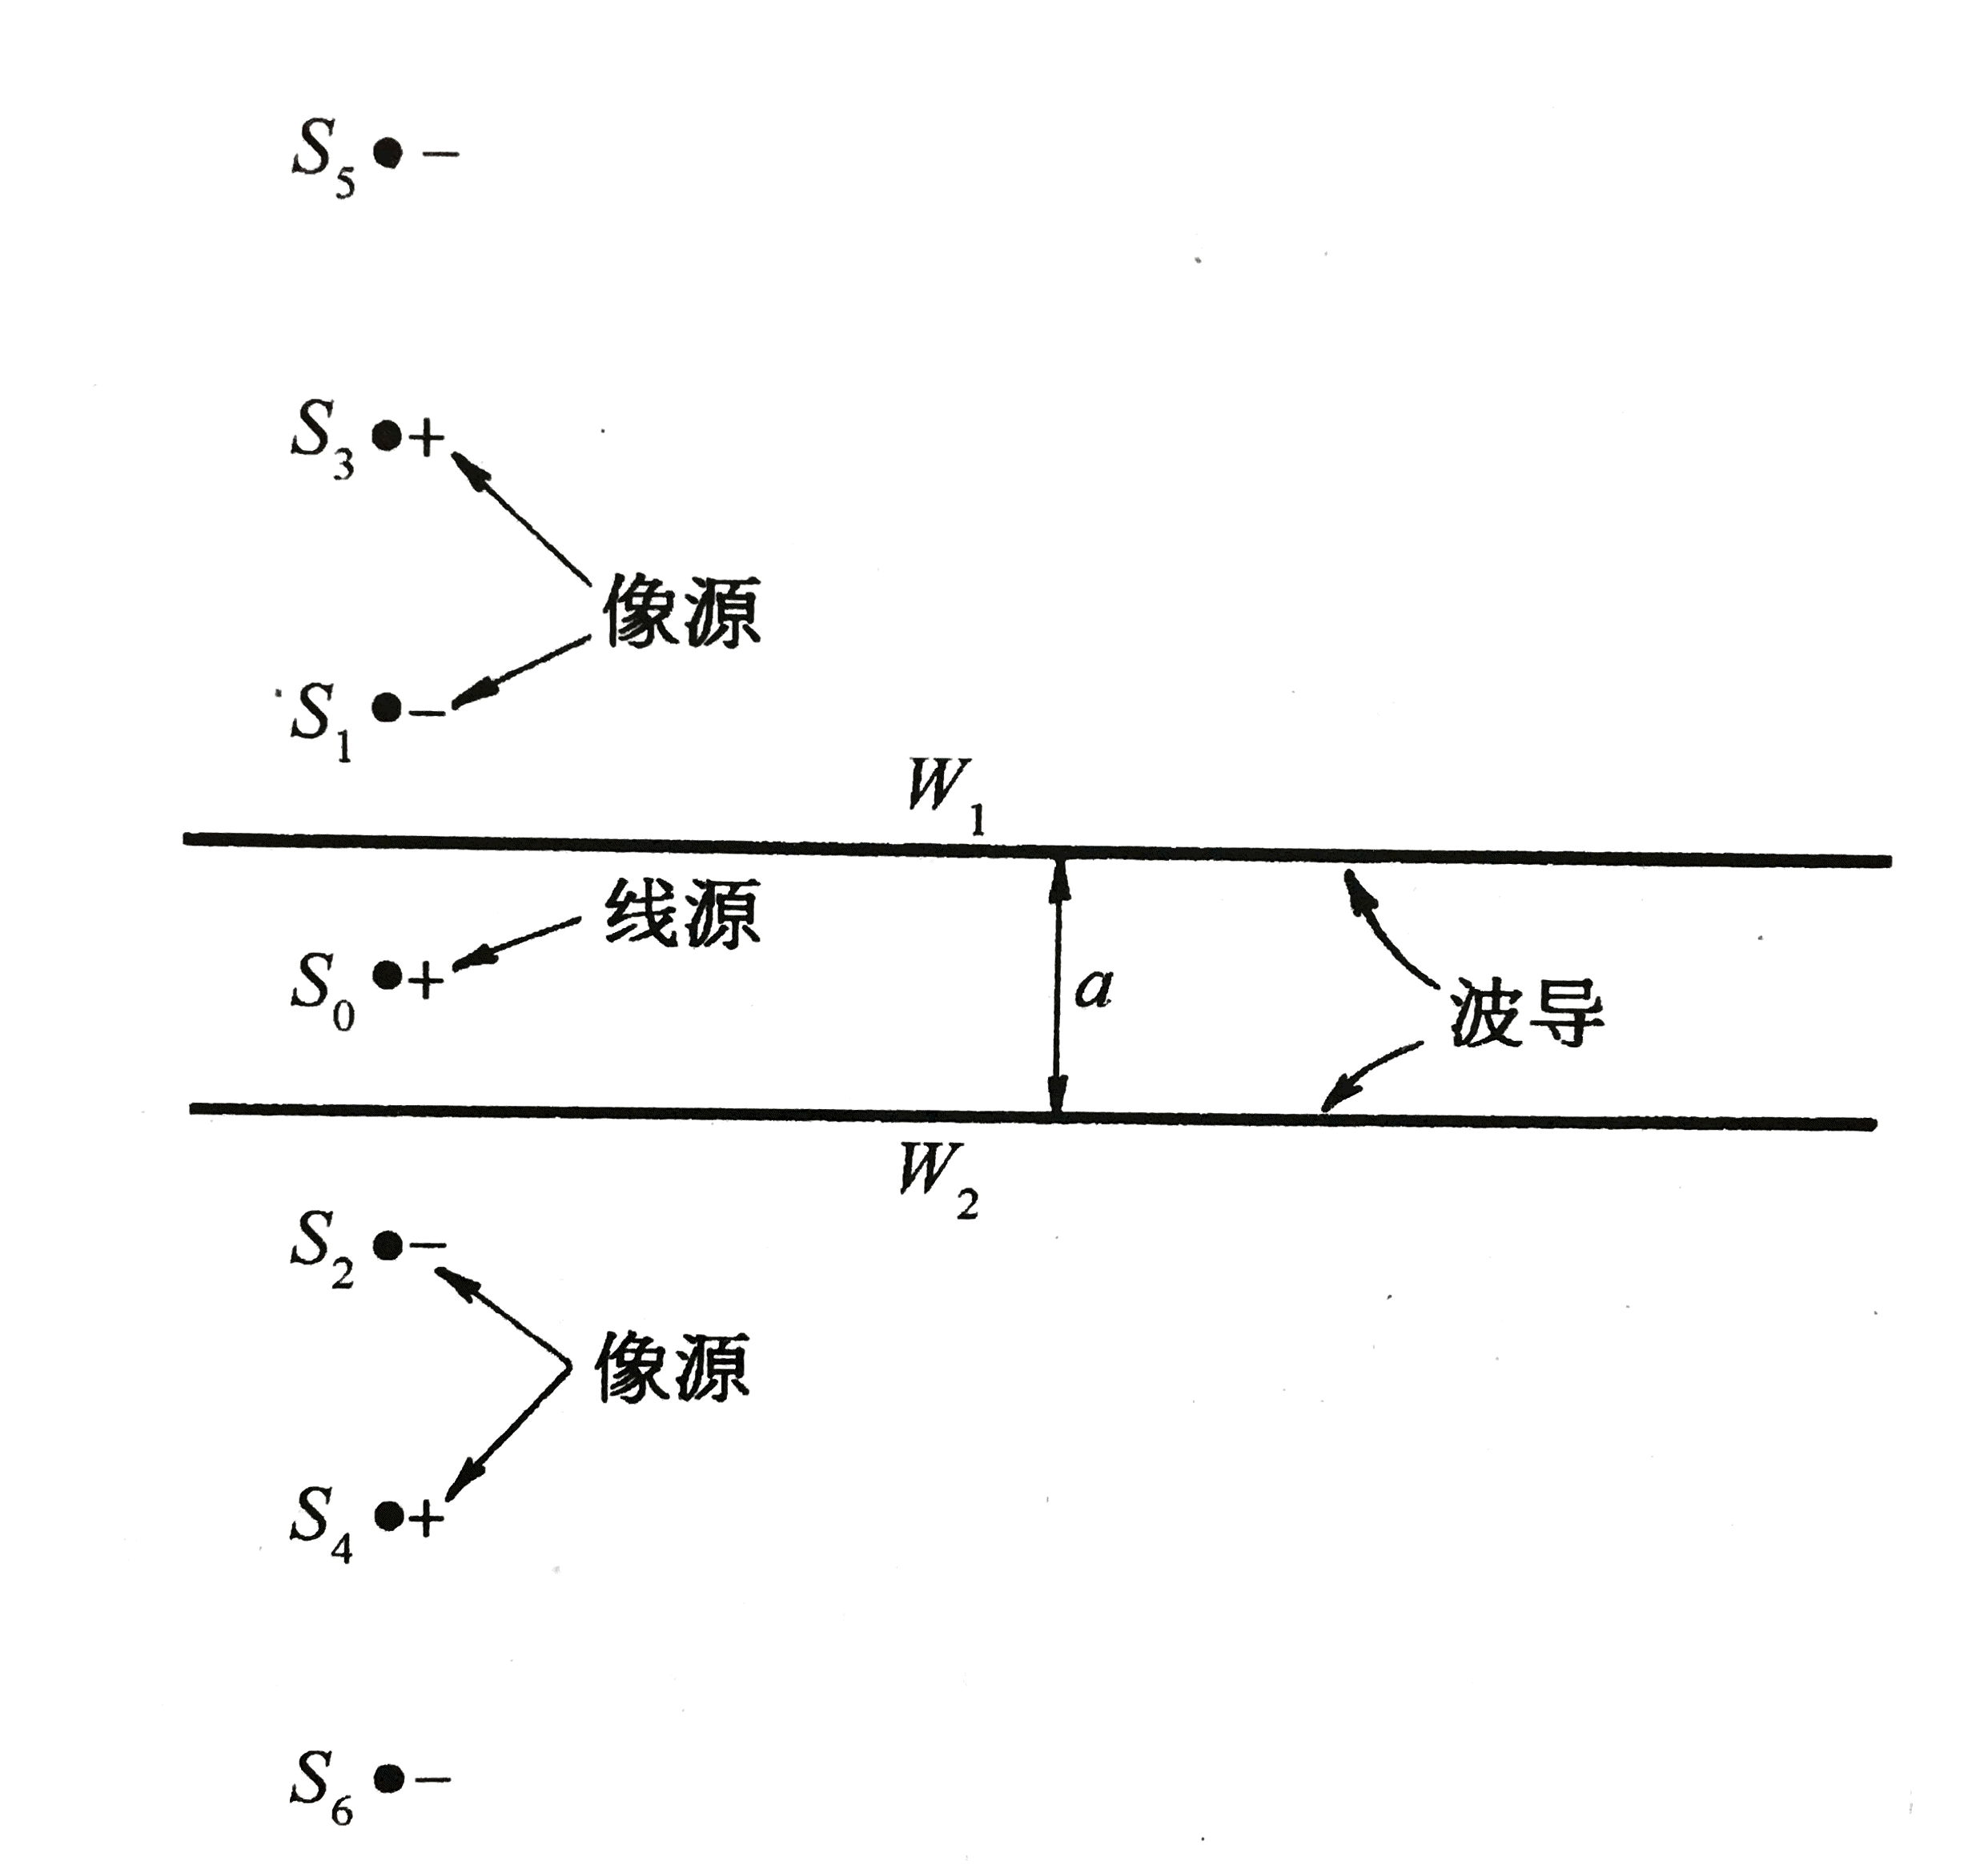
\includegraphics[width=10cm]{0.png}
\caption{放在两面导体臂$W_1$和$W_2$之间的线源$S_0$。这两面壁可以由一个无穷序列的像源代替}
\label{0} 
\end{figure}

我们规定这根元导线里的电流方向为正。现在假如仅有一面壁,比方说$W_1$,我们可以把它除去,只要在那标明为$S_1$的地方放置一个(具有相反极性的)像源。但由于存在两面壁,所以在壁$W_2$中也将有$S_0$的像,将其标为$S_2$。这个像源也将在$W_1$中造成一个像,叫它$S_3$。现在$S_1$和$S_3$两者都将在中在标明为$S_4$和$S_6$的位置上各有其像,如此等等。对于中间有一个源的两个平面导体来说,其场与由排列成一条直线、彼此像个各位$a$的无限多个源所产生的场相同(这事实上就恰如你在观察置于两平行平面镜中间的一根线时所会看到的那样)。为了使在两臂处的场为零,在像上的那些电流极性必须从一个像至另一个像交替地改变着也就是说,它们的振动存在$180^{\circ}$的相位差。于是,该波导场就恰好是这种无限多个线源产生的场的叠加。

如果靠近这些源,场就很像是个静场。这种由一排删型线源所产生的静场,除了随着与删的距离指数减弱的的那些项外,这个场好像一块带点平板产生的场。这里平均源强为零。因为从一个源至下一个源的符号交替改变。任何存在的场会随距离做指数的减弱。在靠近源时,所见到的场主要是来自最接近的源,在较远处,许多源都会做出贡献,因而它们的平均效果便是零了。因此,我们明白了为什么在低于截止频率时波导会给出一个按指数减弱的场。特别是在低频上,这静态近似表现得很好,因而它预言场会随着距离的增大而迅速减弱。

\section{高频时为什么波会传播}

为什么波会传播呢?原因是,在高频时场的推迟会在相位上引进一个附加改变,使得来自那些异相的源的场想长而不是相消。

在图3-1中,观察从那一列像源到达远处的场,只有在某些频率决定的方向——只有在来自所有一切源的场因同相相加的那些方向——场才会最强。在与源有适当距离处,常在这些特殊方向才作为平面波传播。示意图如图3-2所示,其中实线代表波峰而虚线表示波谷。波的传播方向将是这样一个方向:在这个方向两相邻源到达波峰的推迟时差等于半个振动周期,换句话说,图中的$r_2$与$r_0$只差是自由空间波长的一半:
\begin{equation}
	r_2-r_0=\frac{\lambda _0}{2}
\end{equation}

于是角度$\theta$就由下式给出:
\begin{equation}
	sin\theta=\frac{\lambda _0}{2}
\end{equation}

\begin{figure*}
\centering
\begin{minipage}[!htbp]{0.5\textwidth}
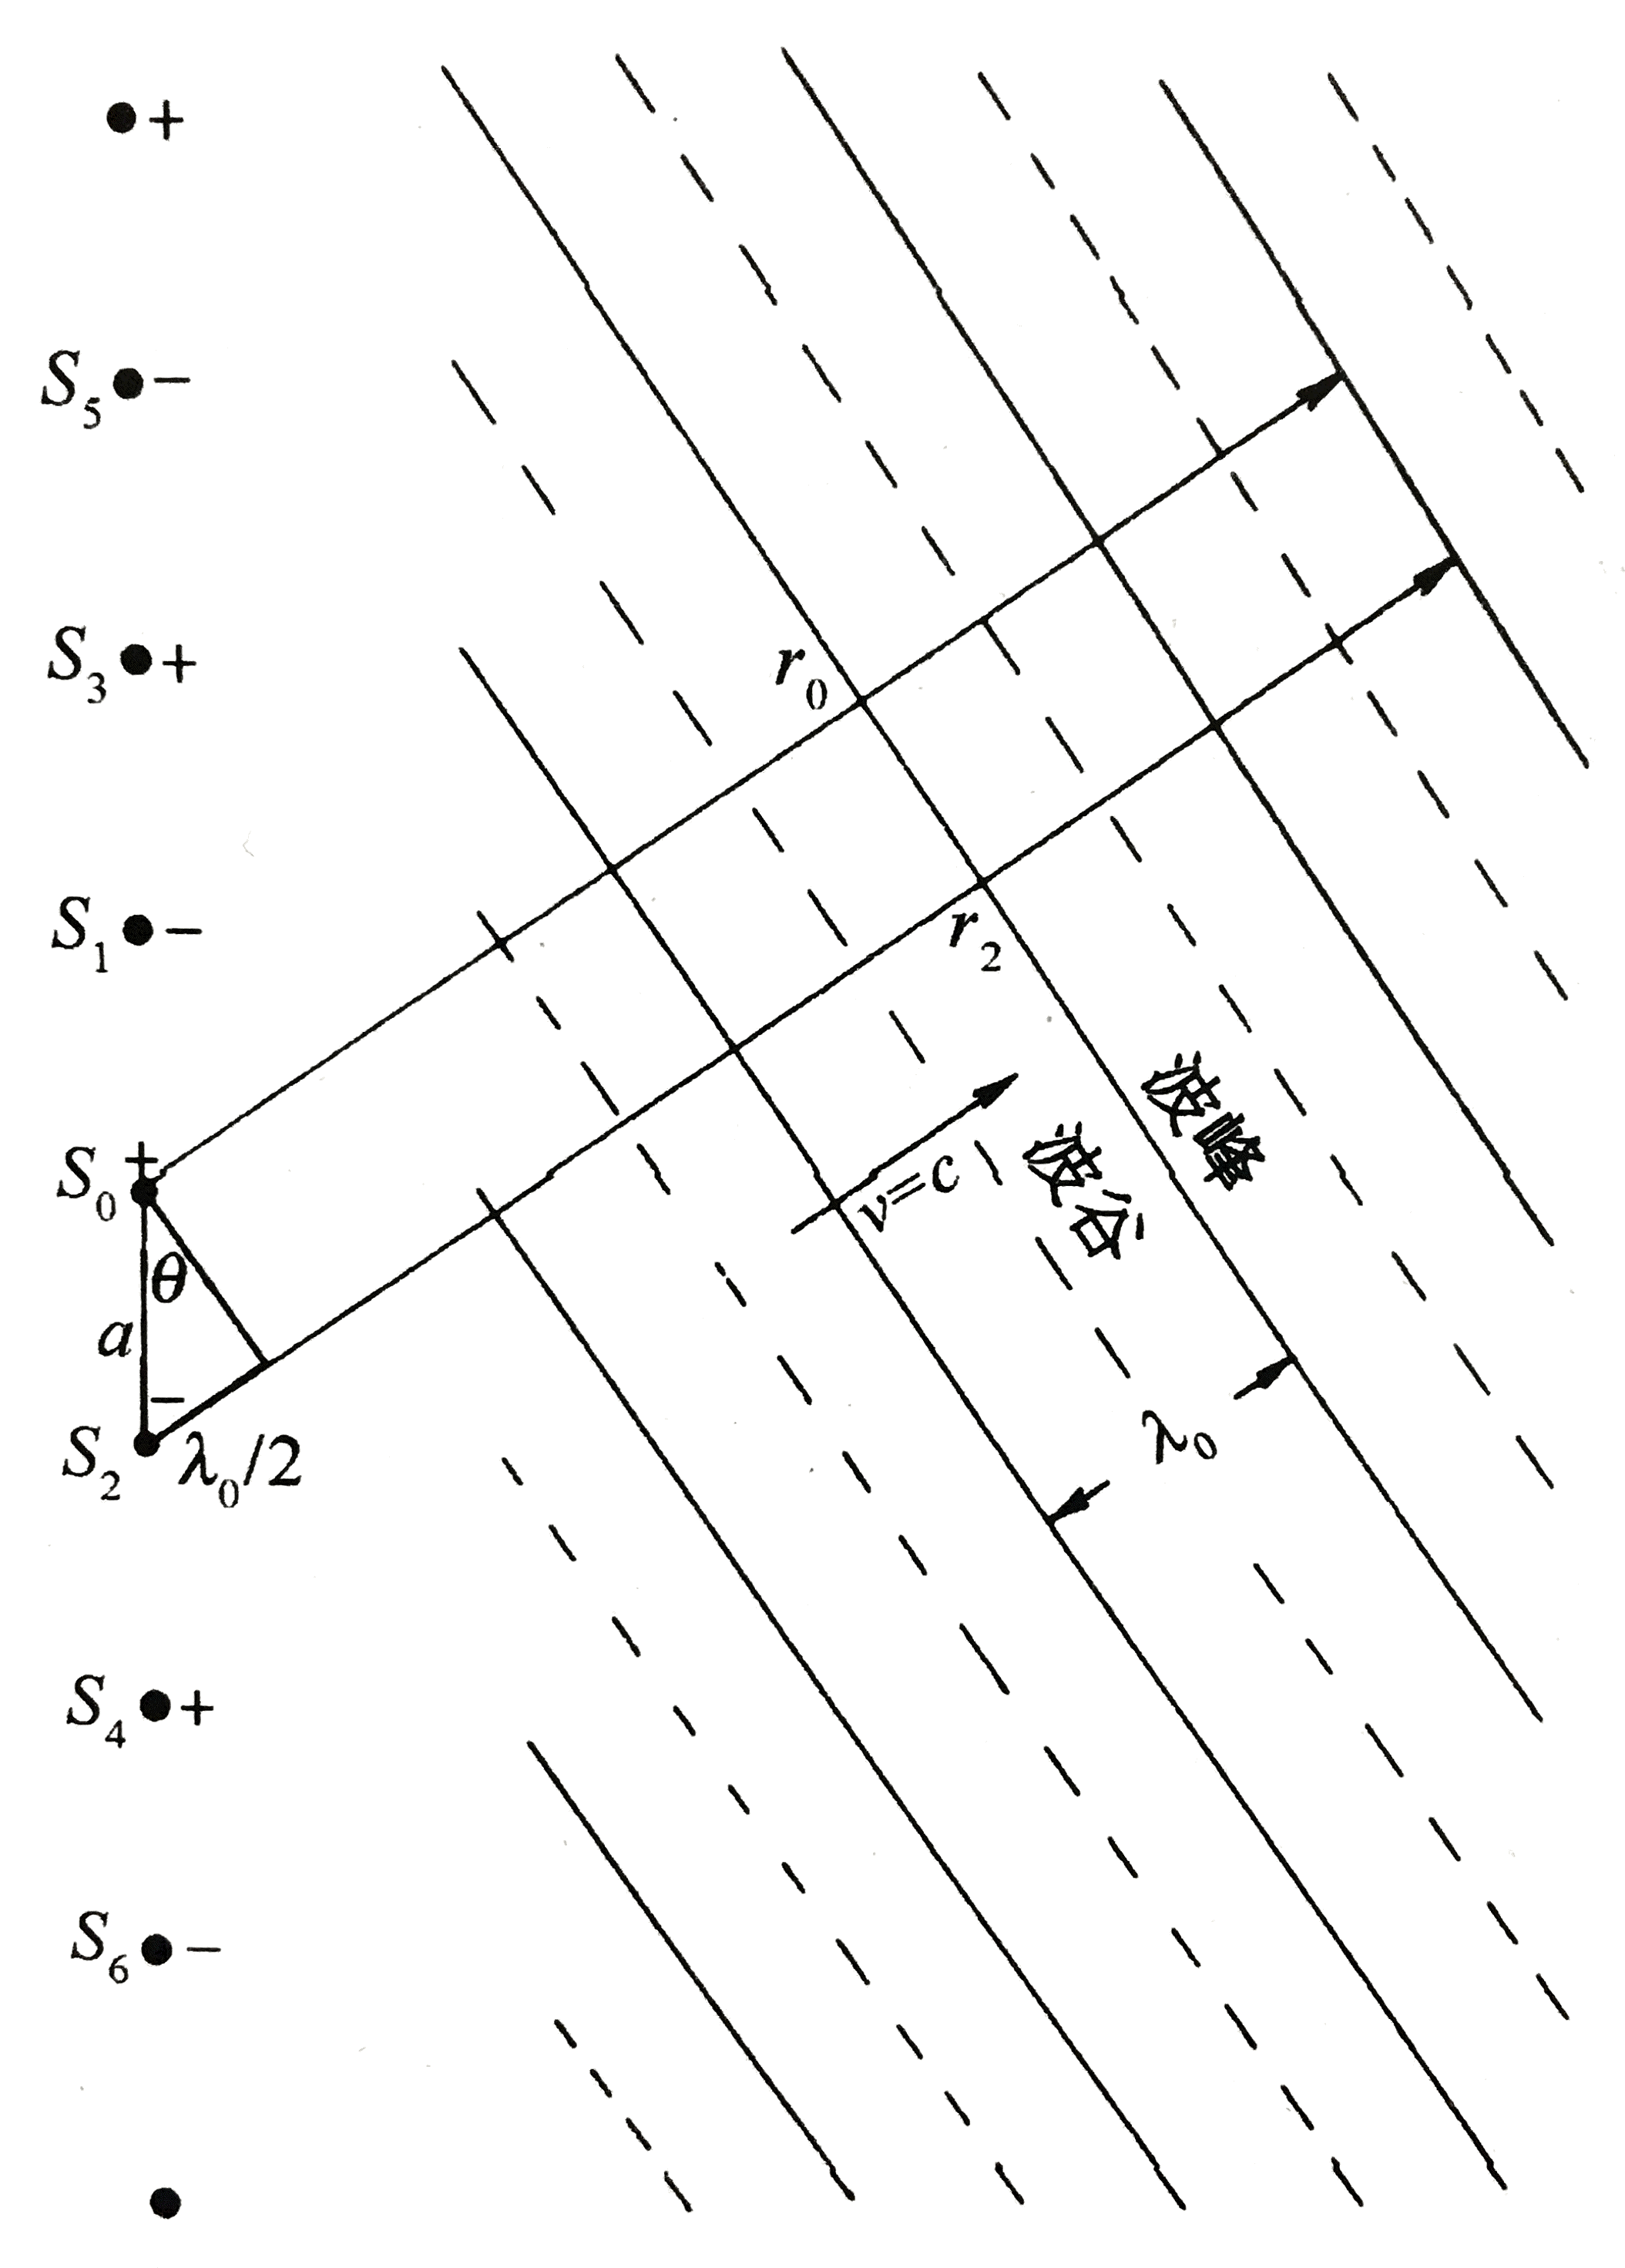
\includegraphics[width=2.2in]{1.png}
\caption{来自一列线源的一组相干波}
\label{fig:side:a}
\end{minipage}%
\begin{minipage}[!htbp]{0.5\textwidth}
\centering
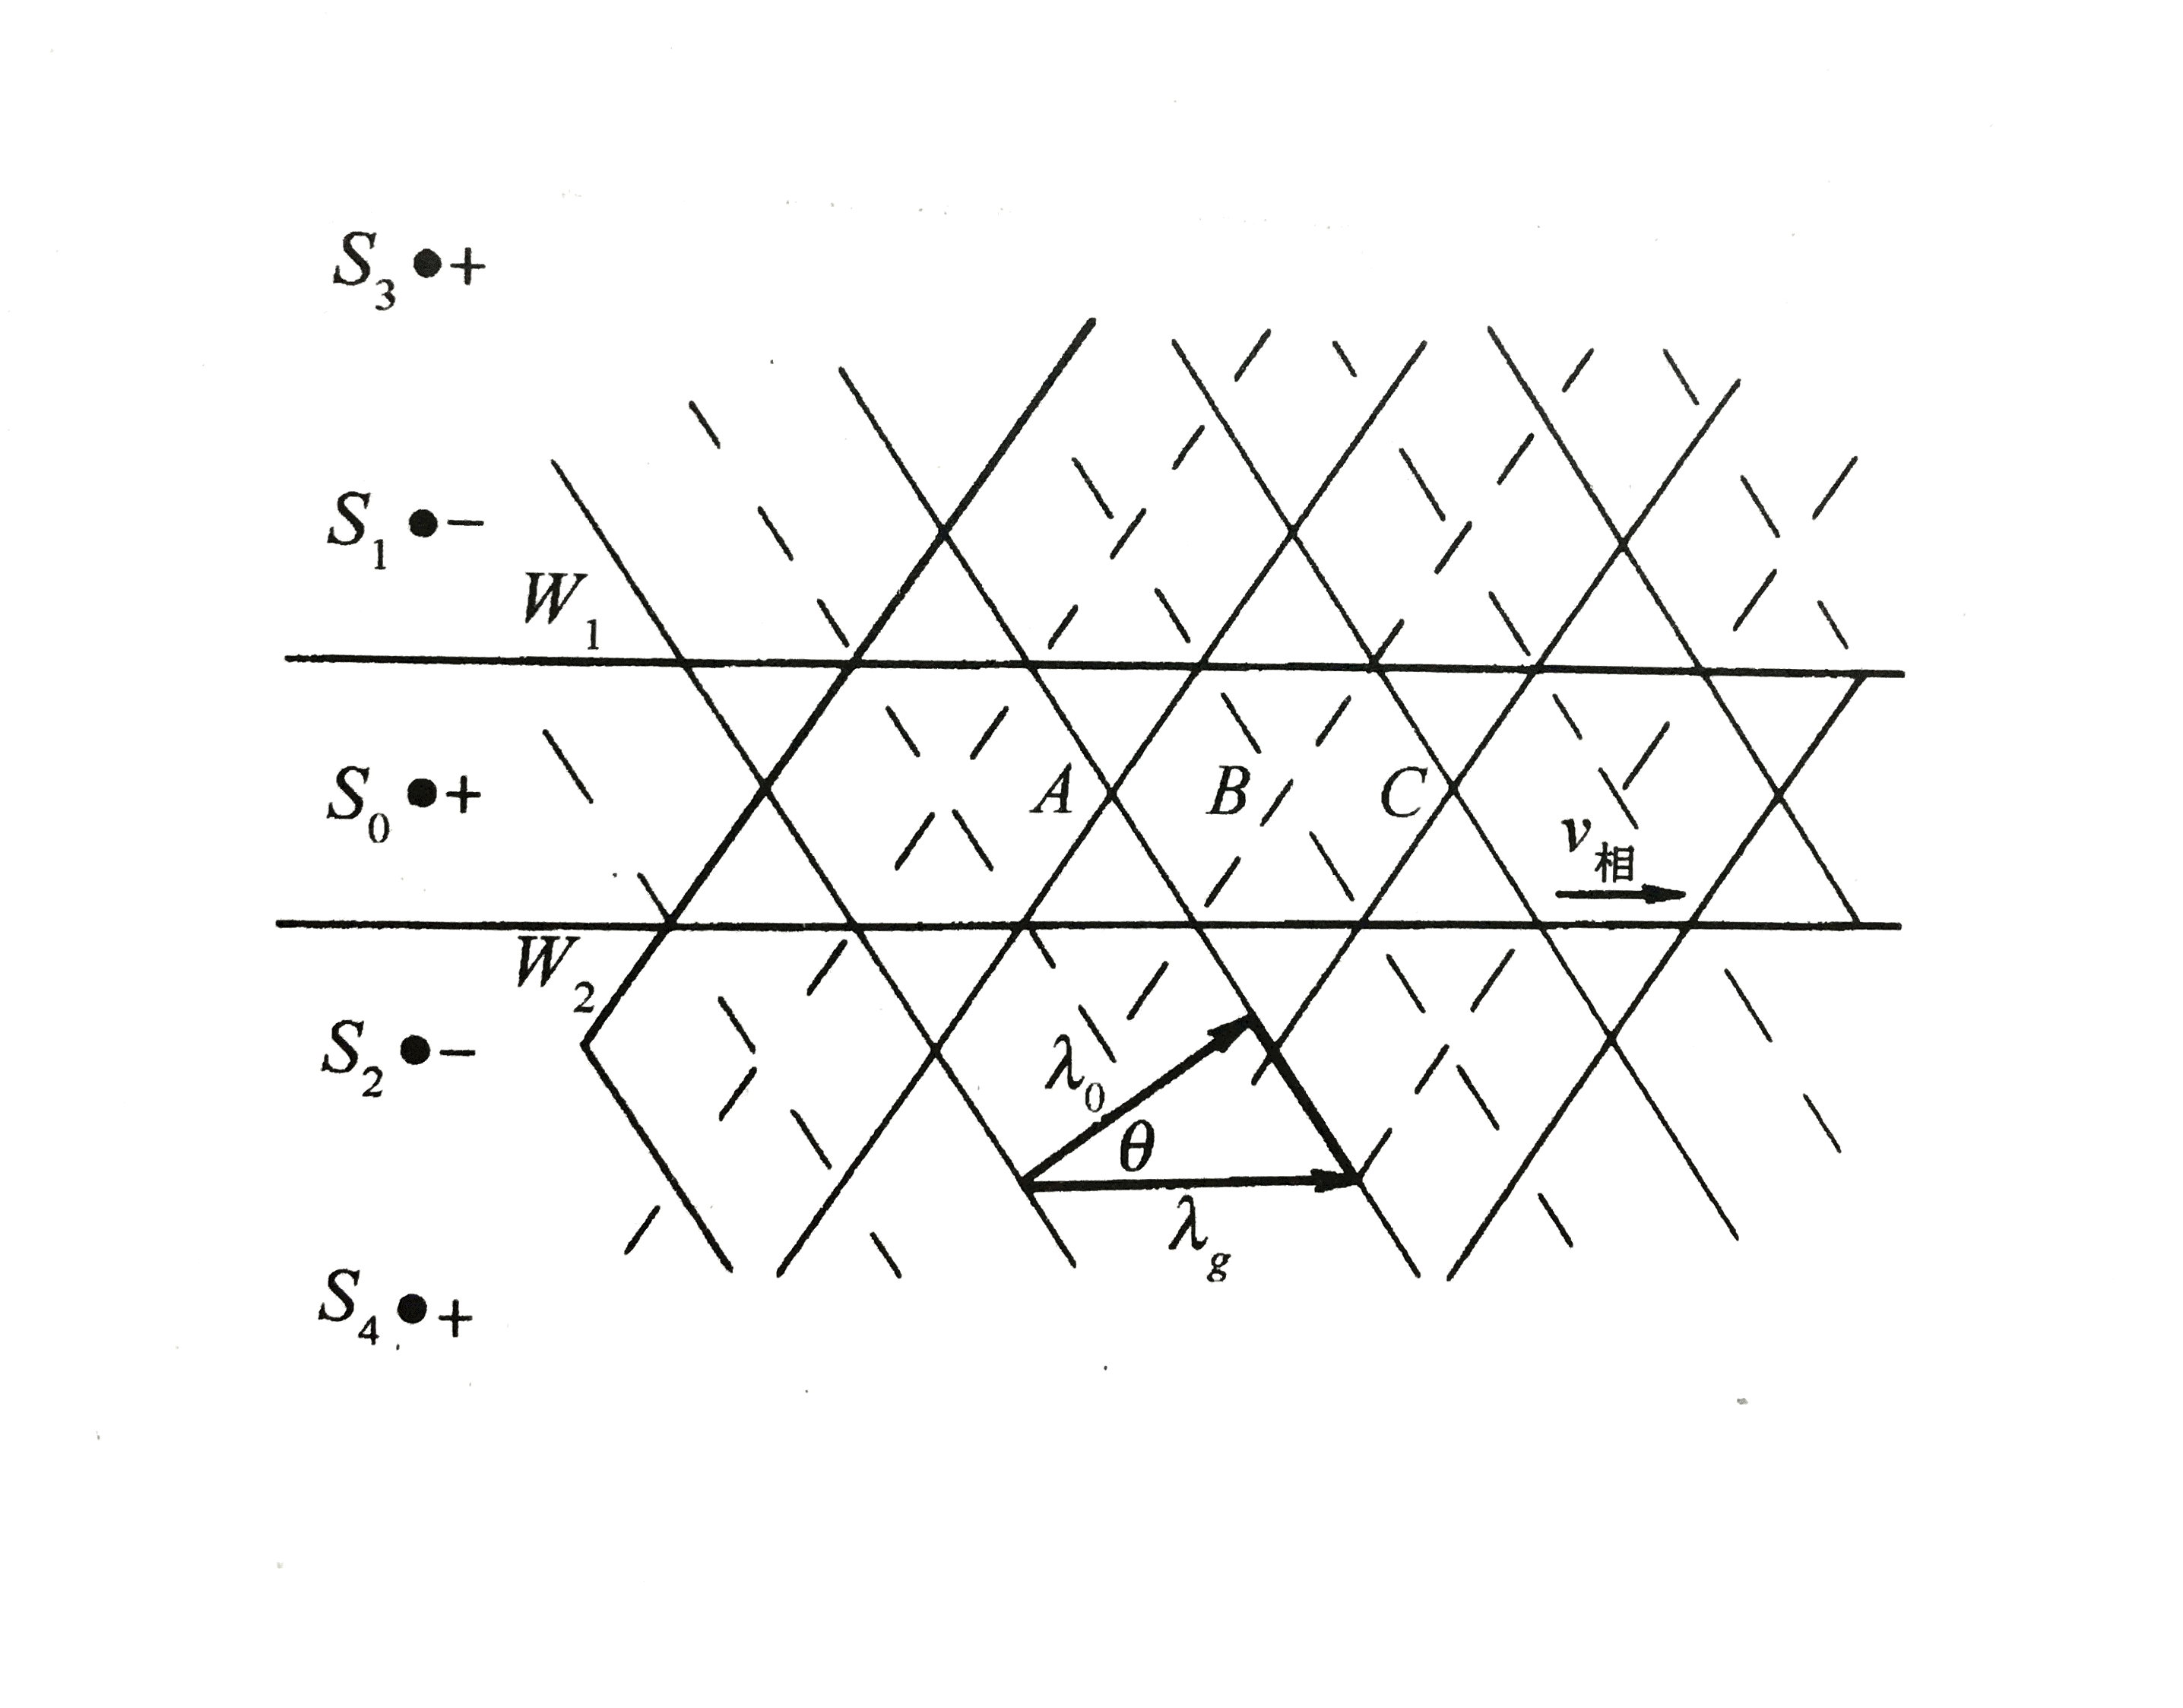
\includegraphics[width=2.2in]{2.png}
\caption{波导场可以视作两列平面波的叠加}
\label{fig:side:b}
\end{minipage}
\end{figure*}
	
当然,还有另一组波以相对于该列线源对称的角度向下传播。整个波导场就是这两组波的叠加,如图(3-3)所示。当然,只有在该波导的两臂之间那实际的场才会真的是这样。

比如在$A$和$C$那些点,两种波形的峰相重合,因而场就有一个极大值;比如在$B$那种点,两波都有负峰值,因而场会有一个极小值(最大负值)。当时间向前推移时,导管里的场会表现出以波长$\lambda _g$——等于从$A$至$C$的距离——沿导管传播。这一距离与角的关系为
\begin{equation}
	cos\theta=\frac{\lambda _0}{\lambda _g}
\end{equation}

利用式(3-2),就可以得到
\begin{equation}
	\lambda _g=\frac{\lambda _0}{cos\theta}=\frac{\lambda _0}{\sqrt{1-{(\lambda _0/2a)^2}}}
\end{equation}

所以这就是为什么只有在超过截止频率是才会有波传播。如果自由空间波长大于2a,则波不能在出现。当$\lambda _0$降至2a以下时,所需的相长干涉才会突然出现。

\section{本章小结}

本章我们将波导描写成无限多个线源的陈列之场的叠加,分别分析了低频高频时波导内场的变化,从而在利用很少的数学公式的情况下,形象化地解释了波导在高、低频之间行为的突然变化。


\chapter{全文总结和课程学习总结}

\section{全文总结}
本文对于波导不能传到TEM波做出了详细多角度的证明,对于波导在高低频之间行为的突变做出了形象化的解释。

\section{课程学习总结}
本学期的电动力学课程,老师们从静电场静磁场到电磁波、相对论,由低频到高频,由浅入深带我们走进了电与磁的世界。在详尽地讲述了理论的同时,还给我们补充了许多点动力学的应用,消除了我们对电动力学的陌生感,让我们对电动力学有了更深刻的认识。这学期的学习让我觉得收获颇丰。


\thesisloadbibliography[nocite]{reference}


\end{document}
